\chapter{Results}
\label{results}
The system was built and tested to prove functionality. After functionality testing was complete, the system was integrated into a 0.60-size Piper Cub R/C aircraft.

\begin{figure}[H]
\label{sysIntPics}
\begin{center}
\begin{minipage}[b]{0.45\linewidth}
  \centering
    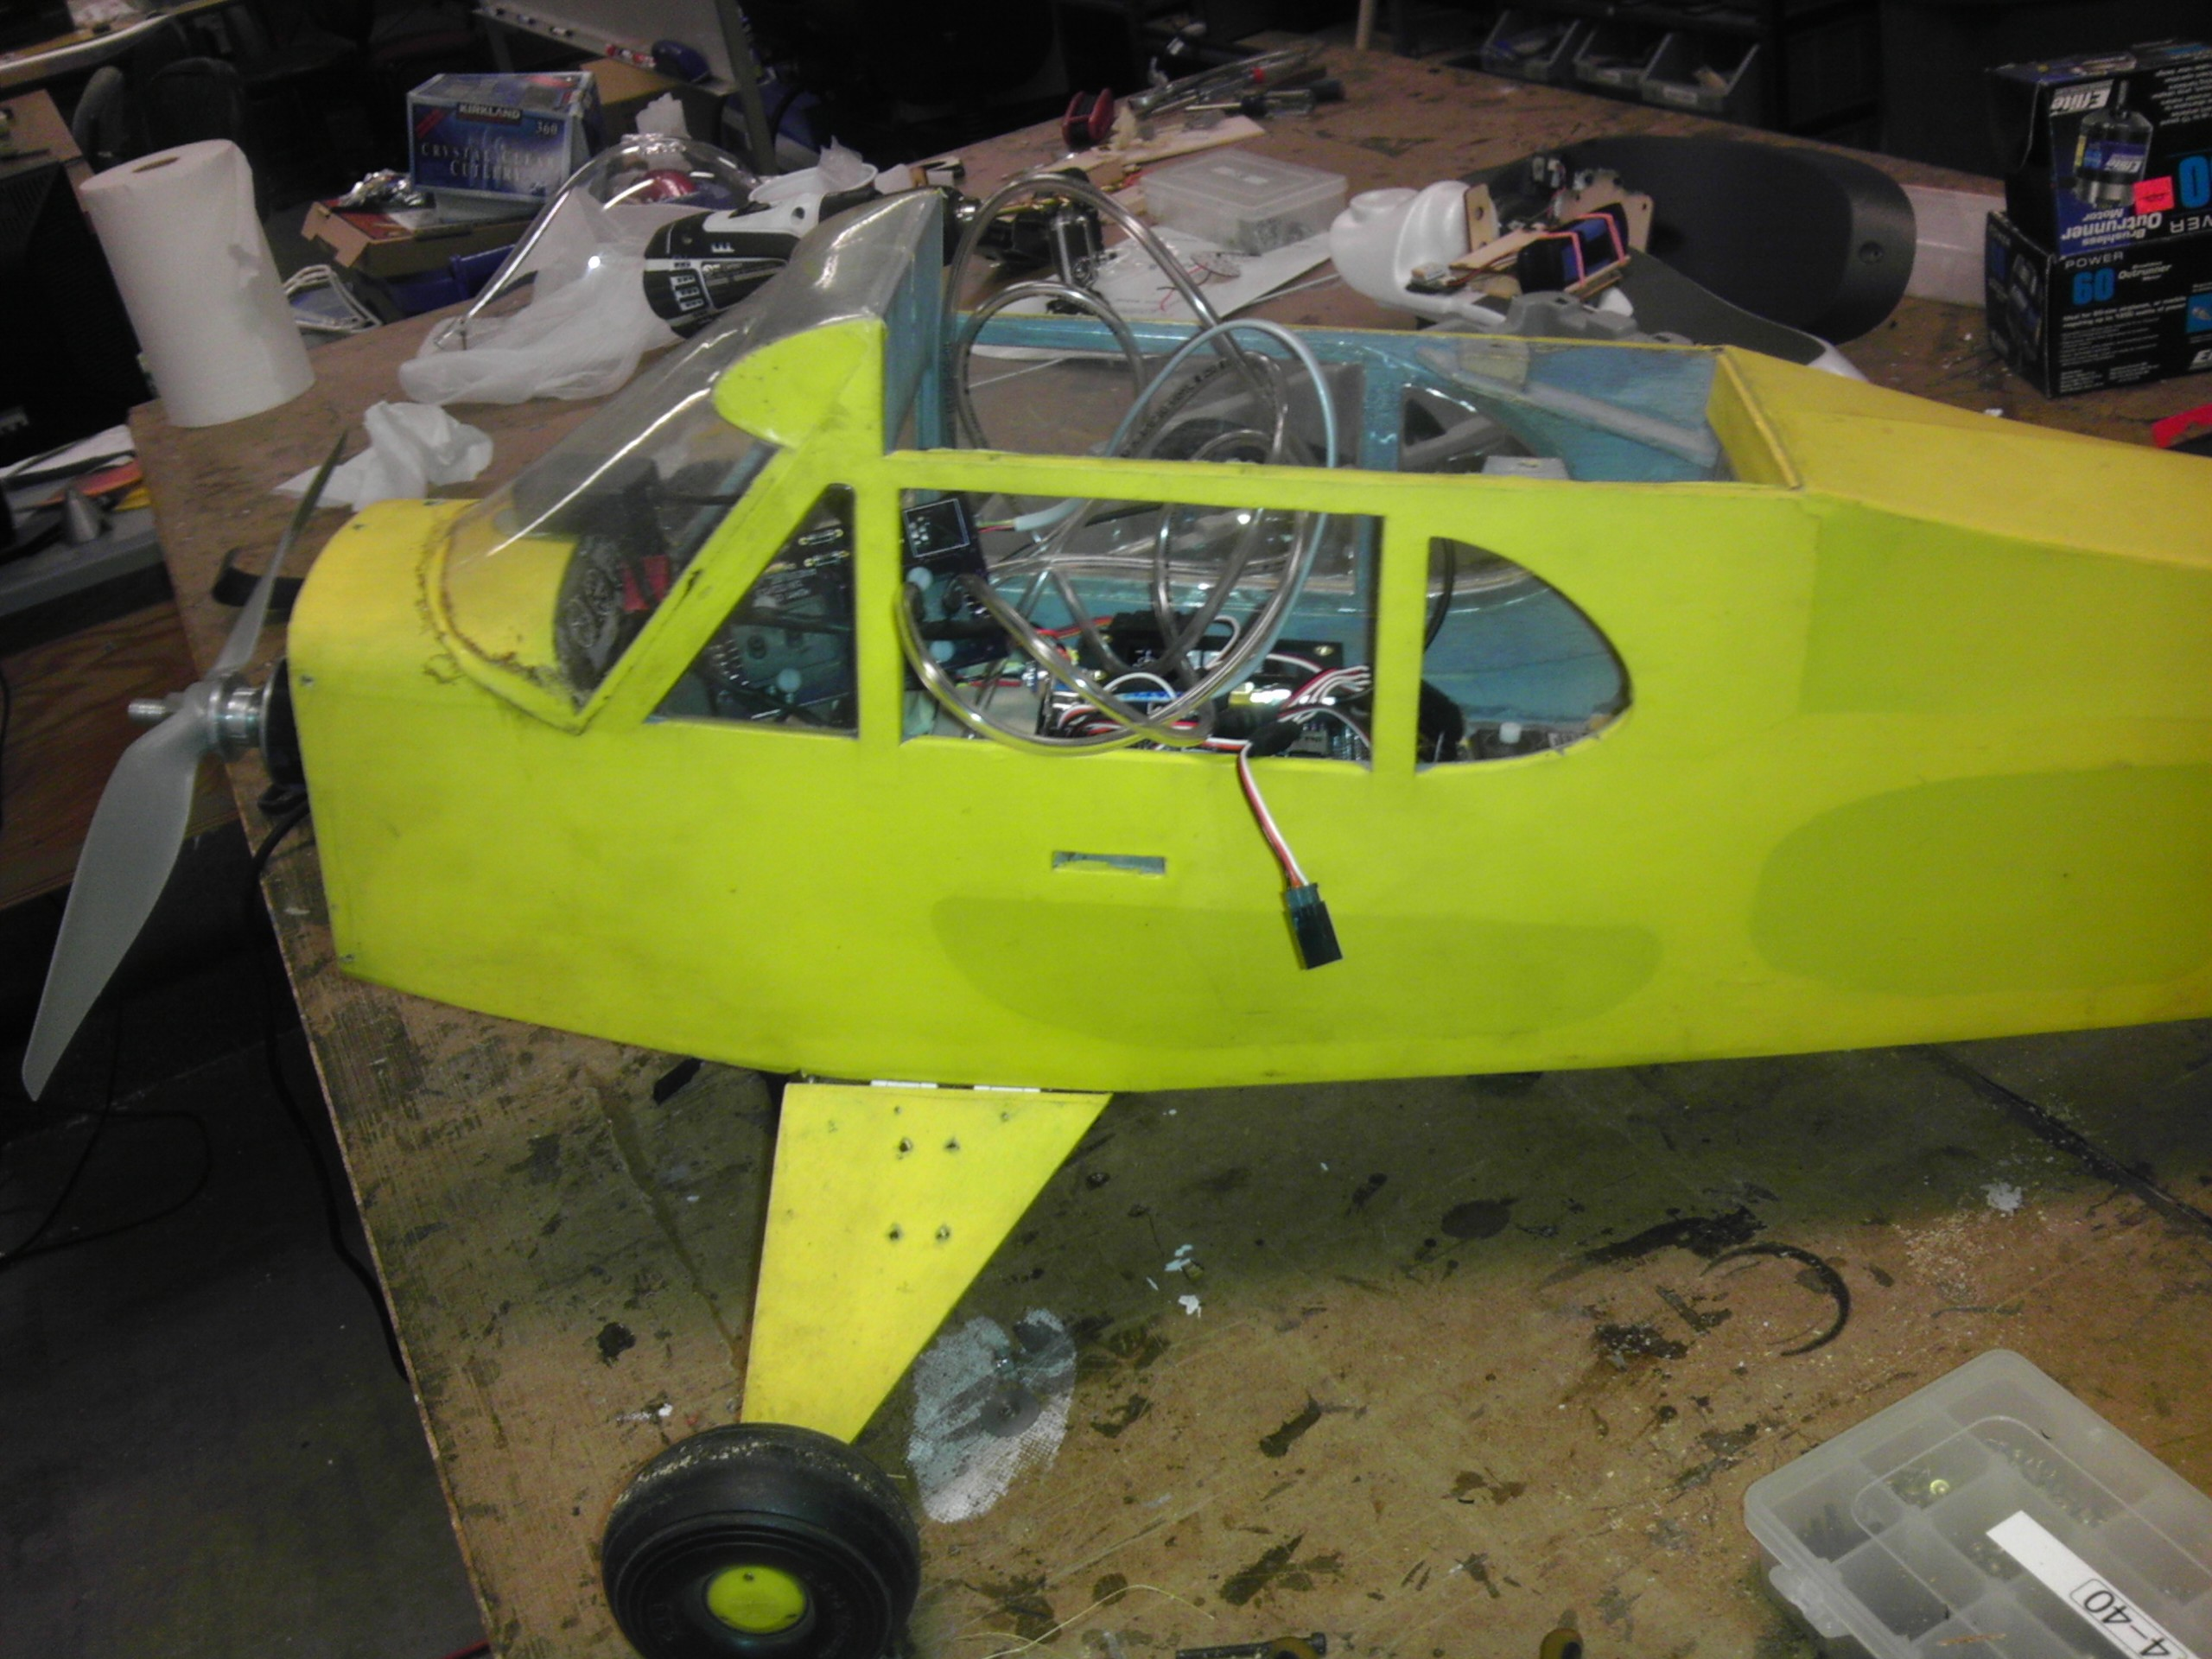
\includegraphics[width=0.9\textwidth]{figures/sysInt1.jpg}
\end{minipage}
\begin{minipage}[b]{0.45\linewidth}
  \centering
    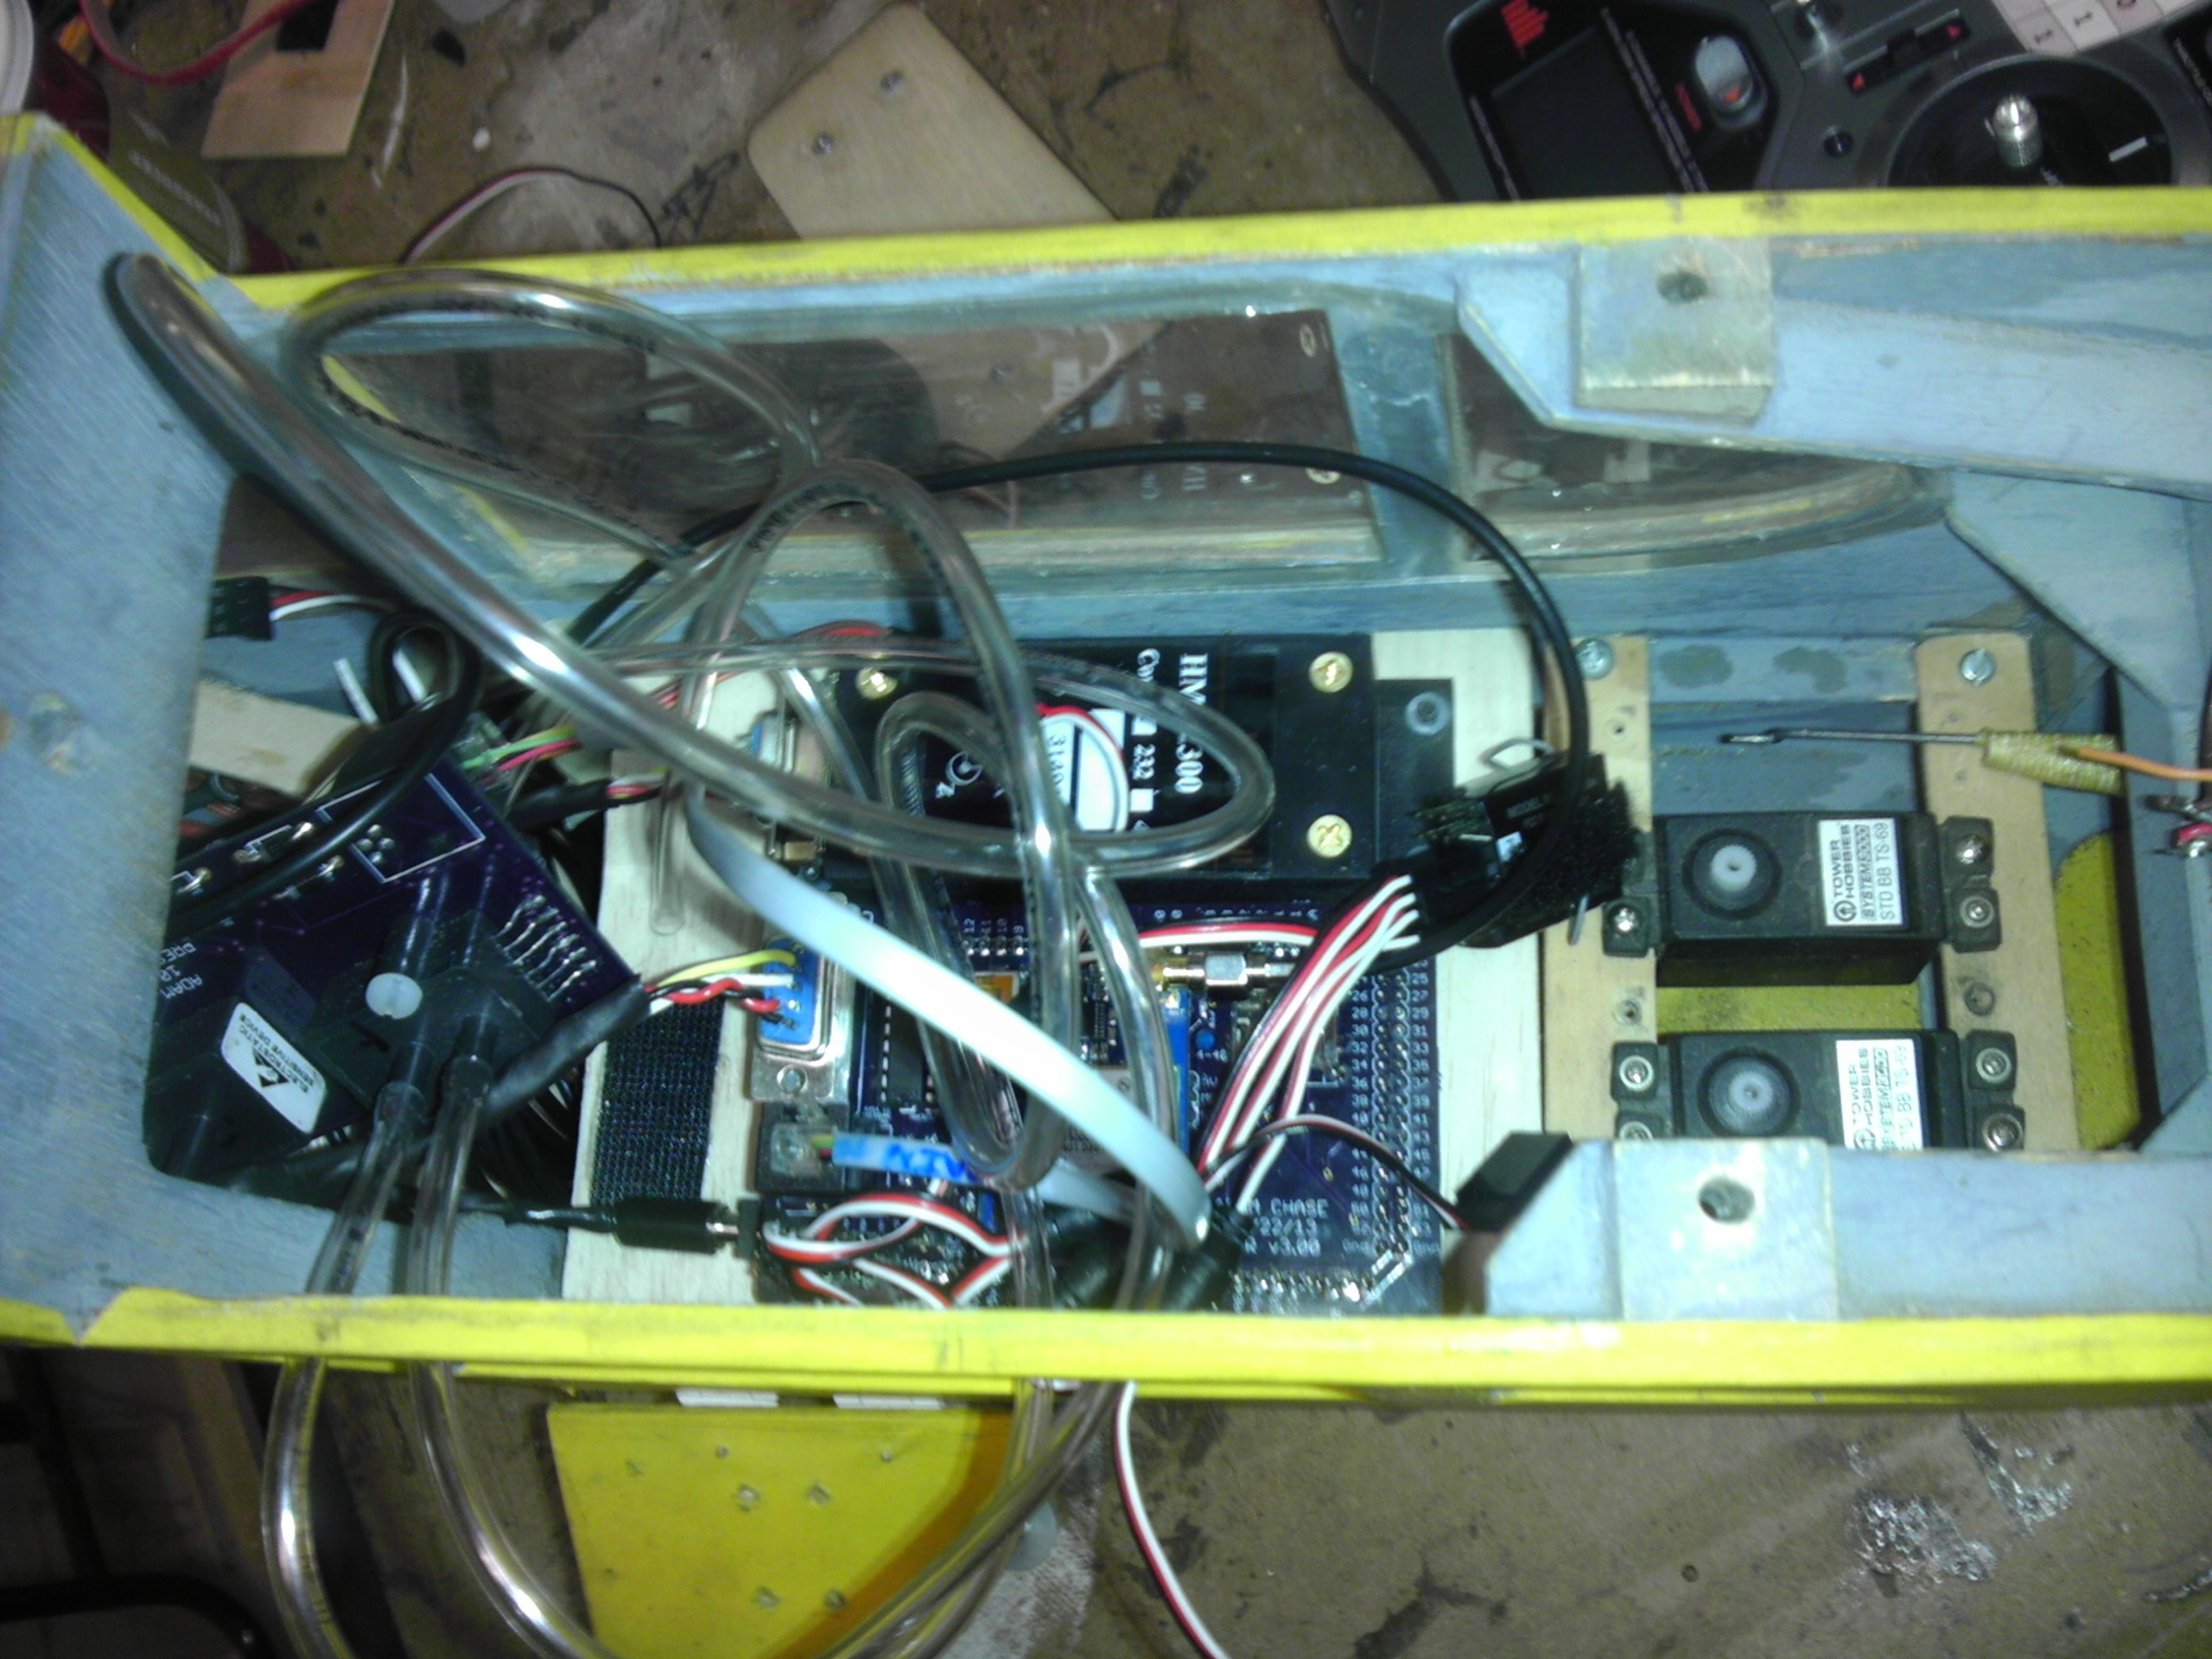
\includegraphics[width=0.9\textwidth]{figures/sysInt2.jpg}
\end{minipage}
\end{center}
\caption{System Integration into 0.60-size R/C Piper Cub}
\end{figure}

Flight testing was completed at Cal Poly's Education Flight Range.\nomenclature[A]{EFR}{Education Flight Range} Each flight test included multiple stalls and high speed dives, so that as much of the flight envelope was covered as possible. More information on specific flight test procedures is available in Appendices \ref{sect:systemUsage} and \ref{sect:flightTestProc}.

\section{Drag Polar}
A drag polar captured from flight data is shown in \ref{fig:flight3PolarErrorBars}. The red lines in figure \ref{fig:flight3PolarErrorBars} are 2-D error bars calculated according to Section \ref{pointErrorSection}.

\begin{figure}[H]
  \centering
    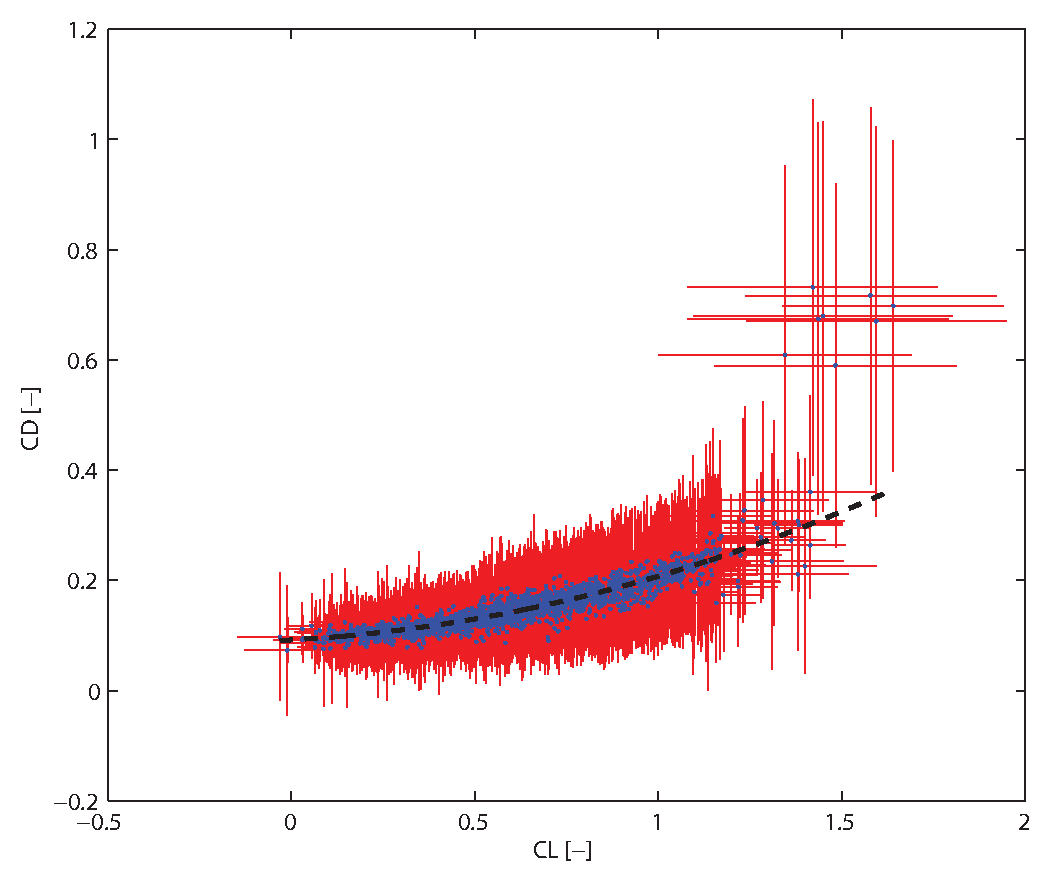
\includegraphics[width=0.7\textwidth]{figures/flight3PolarErrorBars.eps}  \caption{Drag Polar from Flight Test} \label{fig:flight3PolarErrorBars}
\end{figure}
 For this particular flight, the drag polar regression coefficients are shown in Equation \ref{eqn:flight3Polar}.

\begin{align}
\label{eqn:flight3Polar}
C_D &= 0.079243C_L^2 + 0.036290C_L + 0.092005
\end{align}
Sections of particular interest in the drag polar are discussed below.

\subsection{$C_2$ Coefficient}
The wing used on this flight test had a chord of 11.75 inches and a span of 7 feet, which corresponds to an aspect ratio of 7.15. Recalling that the $C_2$ regression coefficient is

\begin{align}
C_2 &= K_1 + K_2
\end{align}
where $K_1$ is the profile drag term from the airfoil, and $K_2$ is the inviscid correction for a finite wing, as shown in Equation \ref{eqn:K2LiftDistribution}.

\begin{align}
\label{eqn:K2LiftDistribution}
K_2 &= \frac{1}{\pi eAR}
\end{align}

Rearranging Equation \ref{eqn:K2LiftDistribution} for the lift distribution $e$ gives

\begin{align}
e &= \frac{1}{\pi AR(C_2-K_1)}.
\end{align}
The $K_1$ term can be found using Equation \ref{eqn:K1Xfoil},
\begin{align}
\label{eqn:K1Xfoil}
K_1 &= \frac{C_1}{-2C_{L_{MIN}}}
\end{align}
where $C_{L_{MIN}}$ is calculated from XFOIL and is 0.26 for the Clark-Y airfoil used. For this flight test, $e = 0.30$. A different method of estimating the lift distribution is also discussed in Section \ref{sect:sysRepeat}.

\subsection{Drag Break}
One of the benefits of the heteroskedastically-robust least squares regression is it's ability to remove outliers from the regression model. This is of substantial benefit when looking at break drag. Break drag is the non-parabolic drag rise that occurs at and past stall. Break drag is evident in Figure \ref{fig:flight3PolarErrorBars}, around $C_L = 1.5$. If the regression model had used an ordinary least squares, the regression scheme would have equally weighted these points and led to an artificially steep parabola. Instead, it's evident that these points past $C_{L_{BREAK}}$ are the only points for which their error bars do not overlap the regression curve.
\subsection{Error Estimation}
One of the key lessons learned from the simulator was that the error in lift and drag prediction is heteroskedastic, and increases as the lift coefficient increases. A plot of the drag polar residuals is shown in \ref{fig:flight3PolarErrorBars}.
\begin{figure}[H]
  \centering
    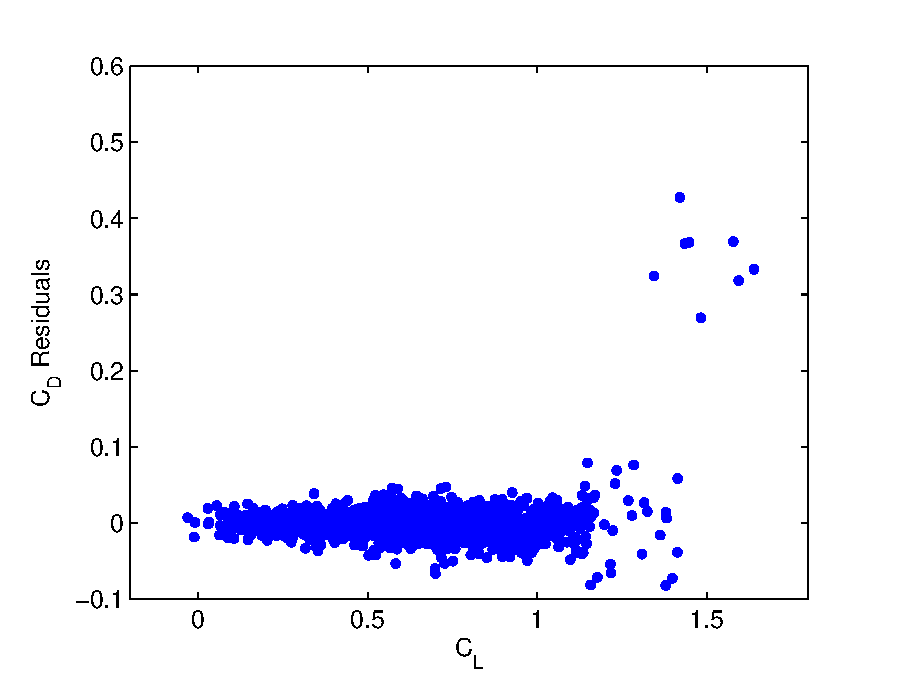
\includegraphics[width=0.7\textwidth]{figures/flight3Residuals.eps}  \caption{Drag Polar Residuals from Flight Test} \label{fig:flight3PolarNoError}
\end{figure}
The scatter of the data matches the trend seen in the simulator. Namely, as $C_L$ goes towards zero, the scatter decreases. This is a direct result of the heteroskedasticity. Since the error is a function of the state, as $C_L$ goes to zero, that contribution of error drops out.
\section{Lift Curve}
A plot of lift coefficient versus angle of attack captured from flight data is shown in \ref{fig:flight3LiftCurve}. Also overlayed is airfoil sectional lift characteristics, taken from XFOIL.
\begin{figure}[H]
  \centering
    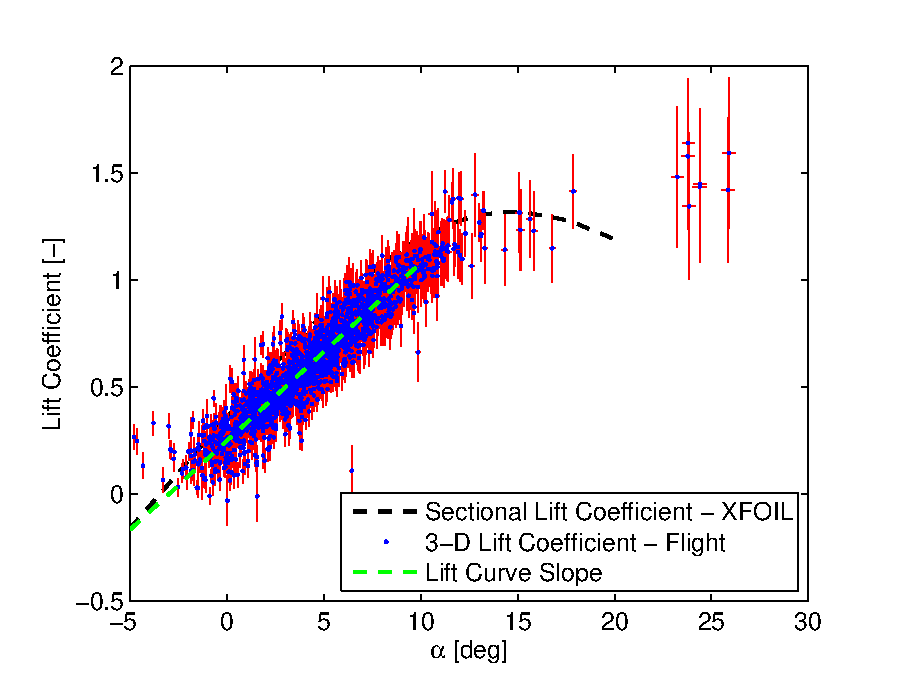
\includegraphics[width=0.7\textwidth]{figures/flight3LiftCurve.eps}  \caption{Lift Curve from Flight Test} \label{fig:flight3LiftCurve}
\end{figure}
Sections of particular interest in the lift curve slope are discussed below.

\subsection{$C_{L_{MAX}}$ and Stall}
Due to the heteroskedastic nature of the error, the error in $C_L$ increases as $C_L$ increases, which makes it particularly difficult to estimate $C_{L_{MAX}}$ with little error. However, the approximate maximum lift coefficient in Figure \ref{fig:flight3LiftCurve} matches well with the estimate of the maximum lift coefficient found using XFOIL. The stall angle of attack appears to be accurate for the set of semi-continuous data. The group of data centered around $\alpha = 25^{\circ}$ is disconnected from the main group of data, as shown Figure \ref{fig:alphaStallHistory}.
\begin{figure}[H]
  \centering
    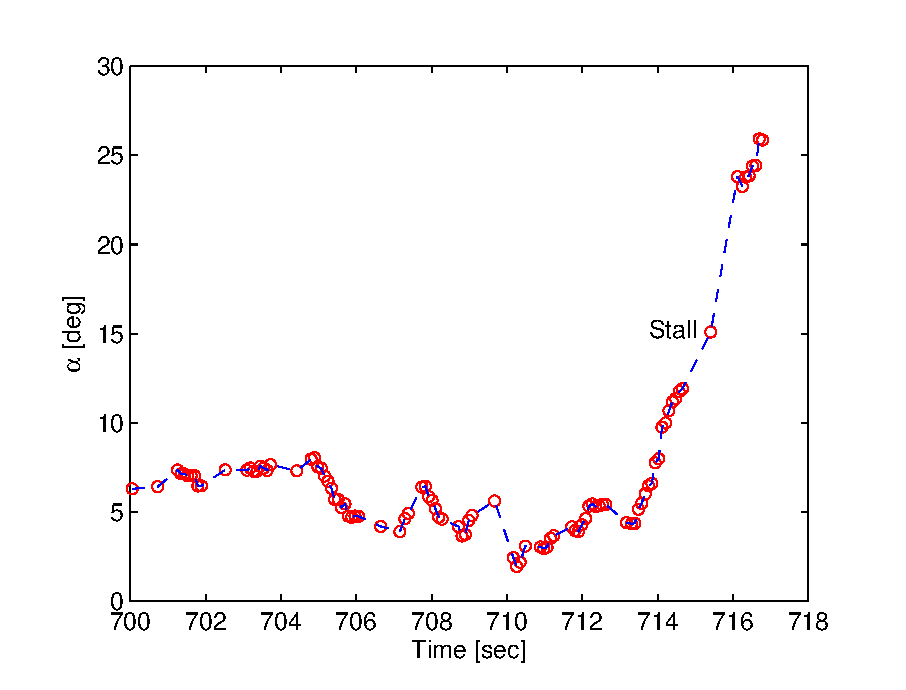
\includegraphics[width=0.7\textwidth]{figures/alphaStallHistory.eps}  \caption{Angle of Attack History from Flight Test} \label{fig:alphaStallHistory}
\end{figure}
The data point at 15 degrees angle of attack corresponds to the stall angle of attack as estimated in XFOIL. After that, a sudden increase in angle of attack occurs as the vehicle stalls. The stall causes the vehicle to rapidly lose altitude, which increases the angle of attack as it falls. This effect causes the discontinuity and makes the original stall angle of attack, which matches that calculated by XFOIL, more accurate.

\subsection{Lift Curve Slope}
The lift curve slope ($C_{l_\alpha}$) of a thin airfoil is 2$\pi$ $C_L$ per radian according to thin airfoil theory. This decreases due to finite wing corrections, and is a function of wing aspect ratio and lift distribution, as shown in Equation \ref{eqn:3dCorrections}

\begin{align}
\label{eqn:3dCorrections}
C_{L_\alpha} &= \frac{C_{l_\alpha}}{1+\frac{C_{l_\alpha}}{\pi e AR}}
\end{align}
where $C_{L_\alpha}$ is the 3-D lift curve slope for the wing. Using the lift distribution found earlier of $e = 0.30$, this gives a 3-D lift curve slope of $C_{L_\alpha} = 3.24$. The slope of the linear regression line in Figure \ref{fig:flight3LiftCurve} is $C_{L_\alpha} = 4.76$, which corresponds to a 32\% error. Again, a different method of estimating this value is presented in Section \ref{sect:sysRepeat}.
\subsection{Zero Lift Angle of Attack}
The 3-D wing corrections only affect the wing when it is producing lift. Therefore, the zero lift angle of attack should stay constant between the 2-D airfoil data analyzed in XFOIL and the 3-D wing data collected in flight. The zero lift angle of attack from XFOIL was -3.0 degrees, and the zero lift angle of attack from flight test was -3.5 degrees.
	
\section{System Repeatability}
\label{sect:sysRepeat}
The system was validated for both repeatability and accuracy. For repeatability, three flight tests were conducted in a clean configuration, and the data was analyzed to verify consistency. A plot of the drag polars from the three flight tests is shown in Figure \ref{fig:dPolarRepeatClean}.

\begin{figure}[H]
  \centering
    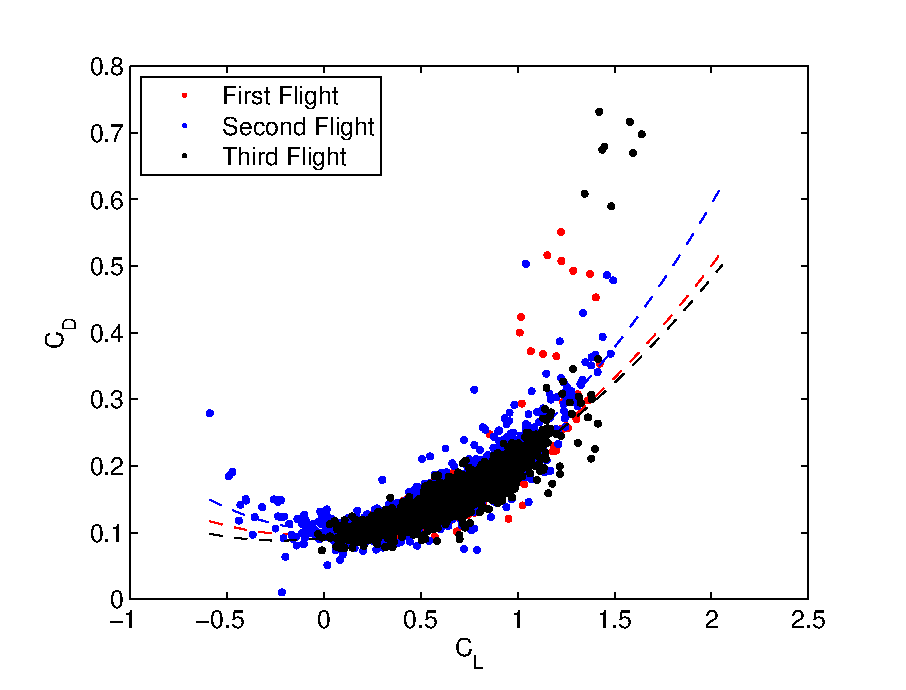
\includegraphics[width=0.8\textwidth]{figures/dPolarRepeatClean.eps}\  \caption{Drag Polar Repeatability Testing} \label{fig:dPolarRepeatClean}
\end{figure}

The estimates of the regression model coefficients for three flight tests are shown in Tables \ref{table:cd0RepeatClean}-\ref{table:k2RepeatClean}.
\newpage
\begin{table}[H]
\caption{Clean Drag Polar Repeatability Testing : $C_{D_0}$ Regression Coefficient}
\label{table:cd0RepeatClean}
\centering
\begin{tabular}{c c c}
\hline\hline
 Flight Number & $C_{D_0}$ Estimate & 95\% Confidence Interval \\
 \hline
1 & 0.097872 &  0.1170/0.0788 \\
2 & 0.103945 & 0.1095/0.0984 \\
3 & 0.092005 & 0.0981/0.0859 \\
\hline \hline
Combined Flights & 0.100037 & 0.1038/0.0963\\
\hline
\end{tabular}
\end{table}

\begin{table}[H]
\caption{Clean Drag Polar Repeatability Testing : $C_1$ Regression Coefficient}
\label{table:c1RepeatClean}
\centering
\begin{tabular}{c c c}
\hline\hline
Flight Number & $C_1$ Estimate & 95\% Confidence Interval \\
 \hline
1 & 0.020783 & 0.0497/-0.0082\\
2 & -0.002644 & 0.0039/-0.0092 \\
3 & 0.036290 & 0.0446/0.0280\\
\hline \hline
Combined Flights & 0.011454 & 0.0163/0.0066\\
\hline
\end{tabular}
\end{table}

\begin{table}[H]
\caption{Clean Drag Polar Repeatability Testing : $C_2$ Regression Coefficient}
\label{table:k2RepeatClean}
\centering
\begin{tabular}{c c c}
\hline\hline
Flight Number & $C_2$ Estimate & 95\% Confidence Interval \\
 \hline
1 & 0.090236 & 0.1009/0.0796 \\
2 & 0.123529 & 0.1255/0.1215 \\
3 & 0.079243 &  0.0819/0.0766\\
\hline \hline
Combined Flights& 0.101002 & 0.1025/0.0995 \\
\hline
\end{tabular}
\end{table}
The parasite drag coefficient was very repeatable for the system. Flights 1 and 3 showed good repeatability for the $C_1$ regression coefficient, but the second flight was an order of magnitude lower. The $C_2$ regression coefficient also showed good repeatability for flights 1 and 3, but was roughly 25\% different for flight 2. This trend is not surprising, since the slope of a linear regression model is more difficult to estimate than the intercept. This is due to there being error in both $C_L$ and $C_D$, and estimating the slope requires multiplying the error in both terms, instead of only the error in $C_D$ for the intercept term.

A plot of the correlation between the regression model and flight test data is shown in Figure \ref{fig:correlationClean}, and a plot of the residuals of the regression model is shown in Figure \ref{fig:residualsClean}.
\begin{figure}[H]
	\centering
	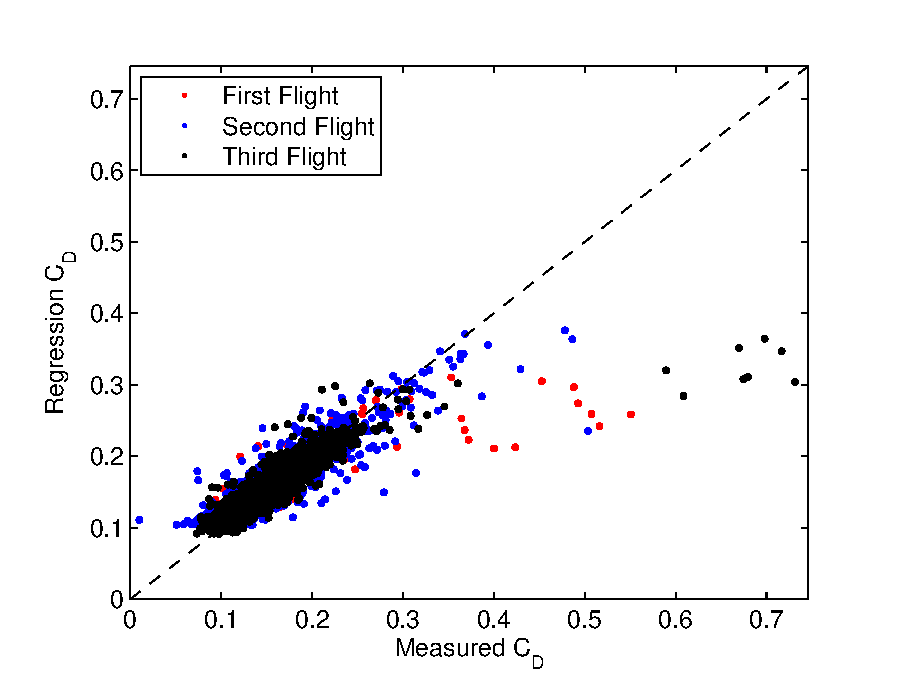
\includegraphics[width=0.7\textwidth]{figures/correlationClean.eps} \caption{Correlation of Regression Model and Flight Data} \label{fig:correlationClean}
\end{figure}
\begin{figure}[H]
	\centering
	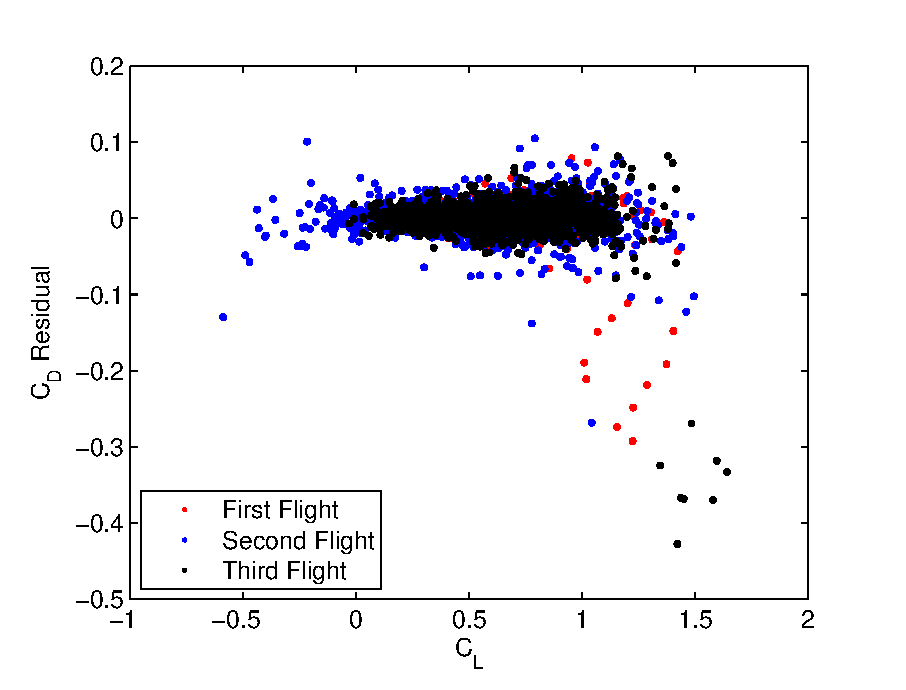
\includegraphics[width=0.7\textwidth]{figures/residualsClean.eps} \caption{Residuals of Regression Model and Flight Data} \label{fig:residualsClean}
\end{figure}
The altered correlation and increased residuals past $C_{L_{BREAK}}$ values was expected, and is a result of using a heteroskedastically-robust estimator. Also note the error increasing on either side of $C_L = 0$, which compares well to the simulator data in Figure \ref{fig:errorBars}.
The system shows similar repeatability for the aircraft's lift characteristics as it does for the drag polar regression. Flight data for three clean flights is shown in Figure \ref{fig:CLalphaRepeatClean}.
\begin{figure}[H]
  \centering
    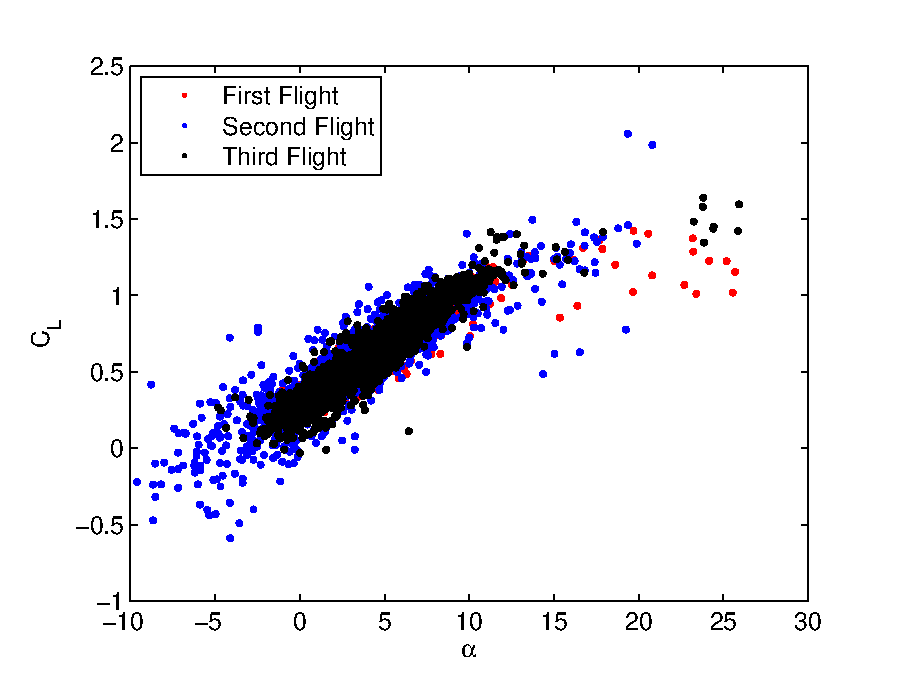
\includegraphics[width=0.7\textwidth]{figures/CLalphaRepeatClean.eps}
      \caption{Lift Curve Repeatability Testing} \label{fig:CLalphaRepeatClean}
\end{figure}

Table \ref{table:liftCurveModel} shows a summary of the zero lift angle of attack. The average zero lift angle of attack is in very good agreement with XFOIL's value of -3.0 degrees.
\begin{table}[H]
\caption{Lift Curve Model}
\label{table:liftCurveModel}
\centering
\begin{tabular}{c c}
\hline\hline
 Flight Number & $\alpha_{0L}$ Estimate \\
 \hline
1 & -2.2$^\circ$\\
2 & -3.4$^\circ$\\
3 & -3.5$^\circ$\\
\hline \hline
Combined Flights & -3.0$^\circ$\\
\hline
\end{tabular}
\end{table}

The scatter in the  $C_1$ and $C_2$ regression coefficients makes estimation of the lift distribution less accurate, as seen with the previously low estimate of $e=0.30$. However, the $C_1$ regression coefficient can be calculated directly using XFOIL, as shown in Figure \ref{fig:clarkYXfoil}. 
\begin{figure}[H]
	\centering
	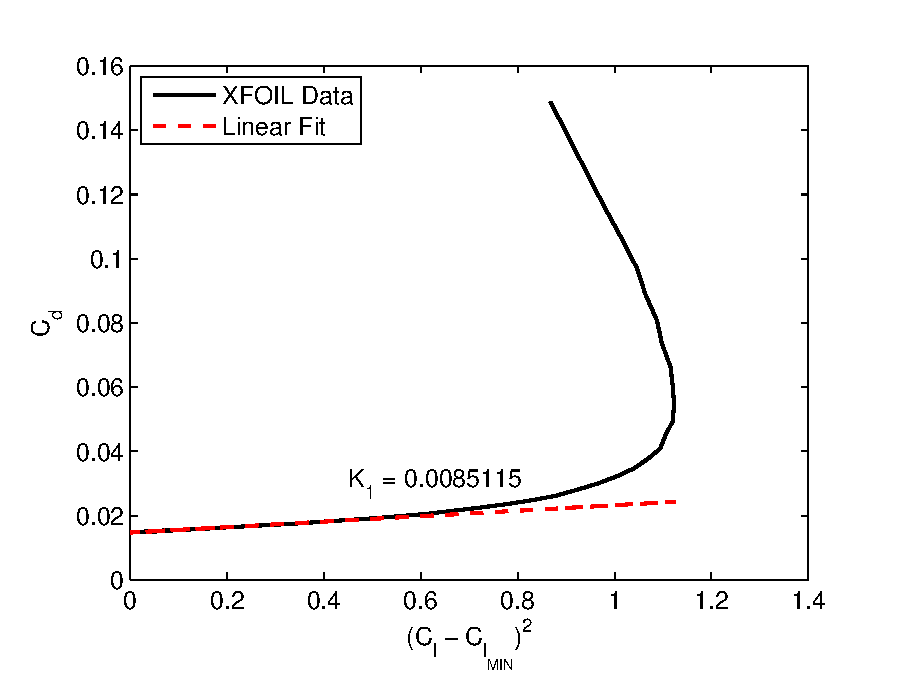
\includegraphics[width=0.7\textwidth]{figures/clarkYXfoil.eps} \caption{XFOIL-based $C_1$ Estimation} \label{fig:clarkYXfoil}
\end{figure}

If that value is used, the estimate of the lift distribution found from flight test data becomes more reasonable, which makes the lift curve slope match better to that estimated by lifting line theory. These results are summarized in Table \ref{table:eXfoil}.

\begin{table}[H]
\caption{Lift Distribution with $C_1$ From Flight and XFOIL}
\label{table:eXfoil}
\centering
\begin{tabular}{c c c c c}
\hline\hline
 Flight Number & \multicolumn{2}{c}{$C_1$} & \multicolumn{2}{c}{$e$ Estimate}\\
 \hline
 & Flight & XFOIL & Flight& XFOIL\\
1 & 0.020783 & 0.0085115 & 0.34 & 0.54\\
2 & -0.002644& 0.0085115 & 0.38 & 0.39\\
3 & 0.036290 & 0.0085115  & 0.30 & 0.63\\
\hline \hline
Combined Flights & 0.011454 & 0.36 & &0.48\\
\hline
\end{tabular}
\end{table}
The lift distributions from Table \ref{table:eXfoil} were used in Equation \ref{eqn:3dCorrections}, and the results are shown in Table \ref{table:CLAlphaXfoil}.
\begin{table}[H]
\caption{Lift Curve Slope with $C_1$ From Flight and XFOIL}
\label{table:CLAlphaXfoil}
\centering
\begin{tabular}{c c c c c c c}
\hline\hline
 Flight Number & \multicolumn{2}{c}{$C_1$} & \multicolumn{2}{c}{$C_{L_\alpha}$ Estimate} & \multicolumn{2}{c}{$Percent Error$}\\
 \hline
 & Flight & XFOIL & Flight& XFOIL & Flight & XFOIL\\
1 & 0.020783 & 0.0085115 & 3.46 & 4.15 & 27 & 13\\
2 & -0.002644 & 0.0085115 &  3.60&  3.65 & 24 & 23\\
3 & 0.036290 & 0.0085115  &  3.24 & 4.35 & 32 & 9\\
\hline \hline
Combined Flights & 0.011454 & 0.0085115 & 4.76 & 3.9738 & 25 & 16\\
\hline
\end{tabular}
\end{table}

\section{System Accuracy}
The accuracy of the system was validated by adding additional parasite drag of a known amount and measuring the difference in the vehicle's parasite drag coefficient. This was accomplished using a cone that was trailed behind the aircraft, shown in Figure \ref{fig:coneIntegration}. 

\begin{figure}[H]
\begin{center}
\begin{minipage}[b]{0.45\linewidth}
  \centering
    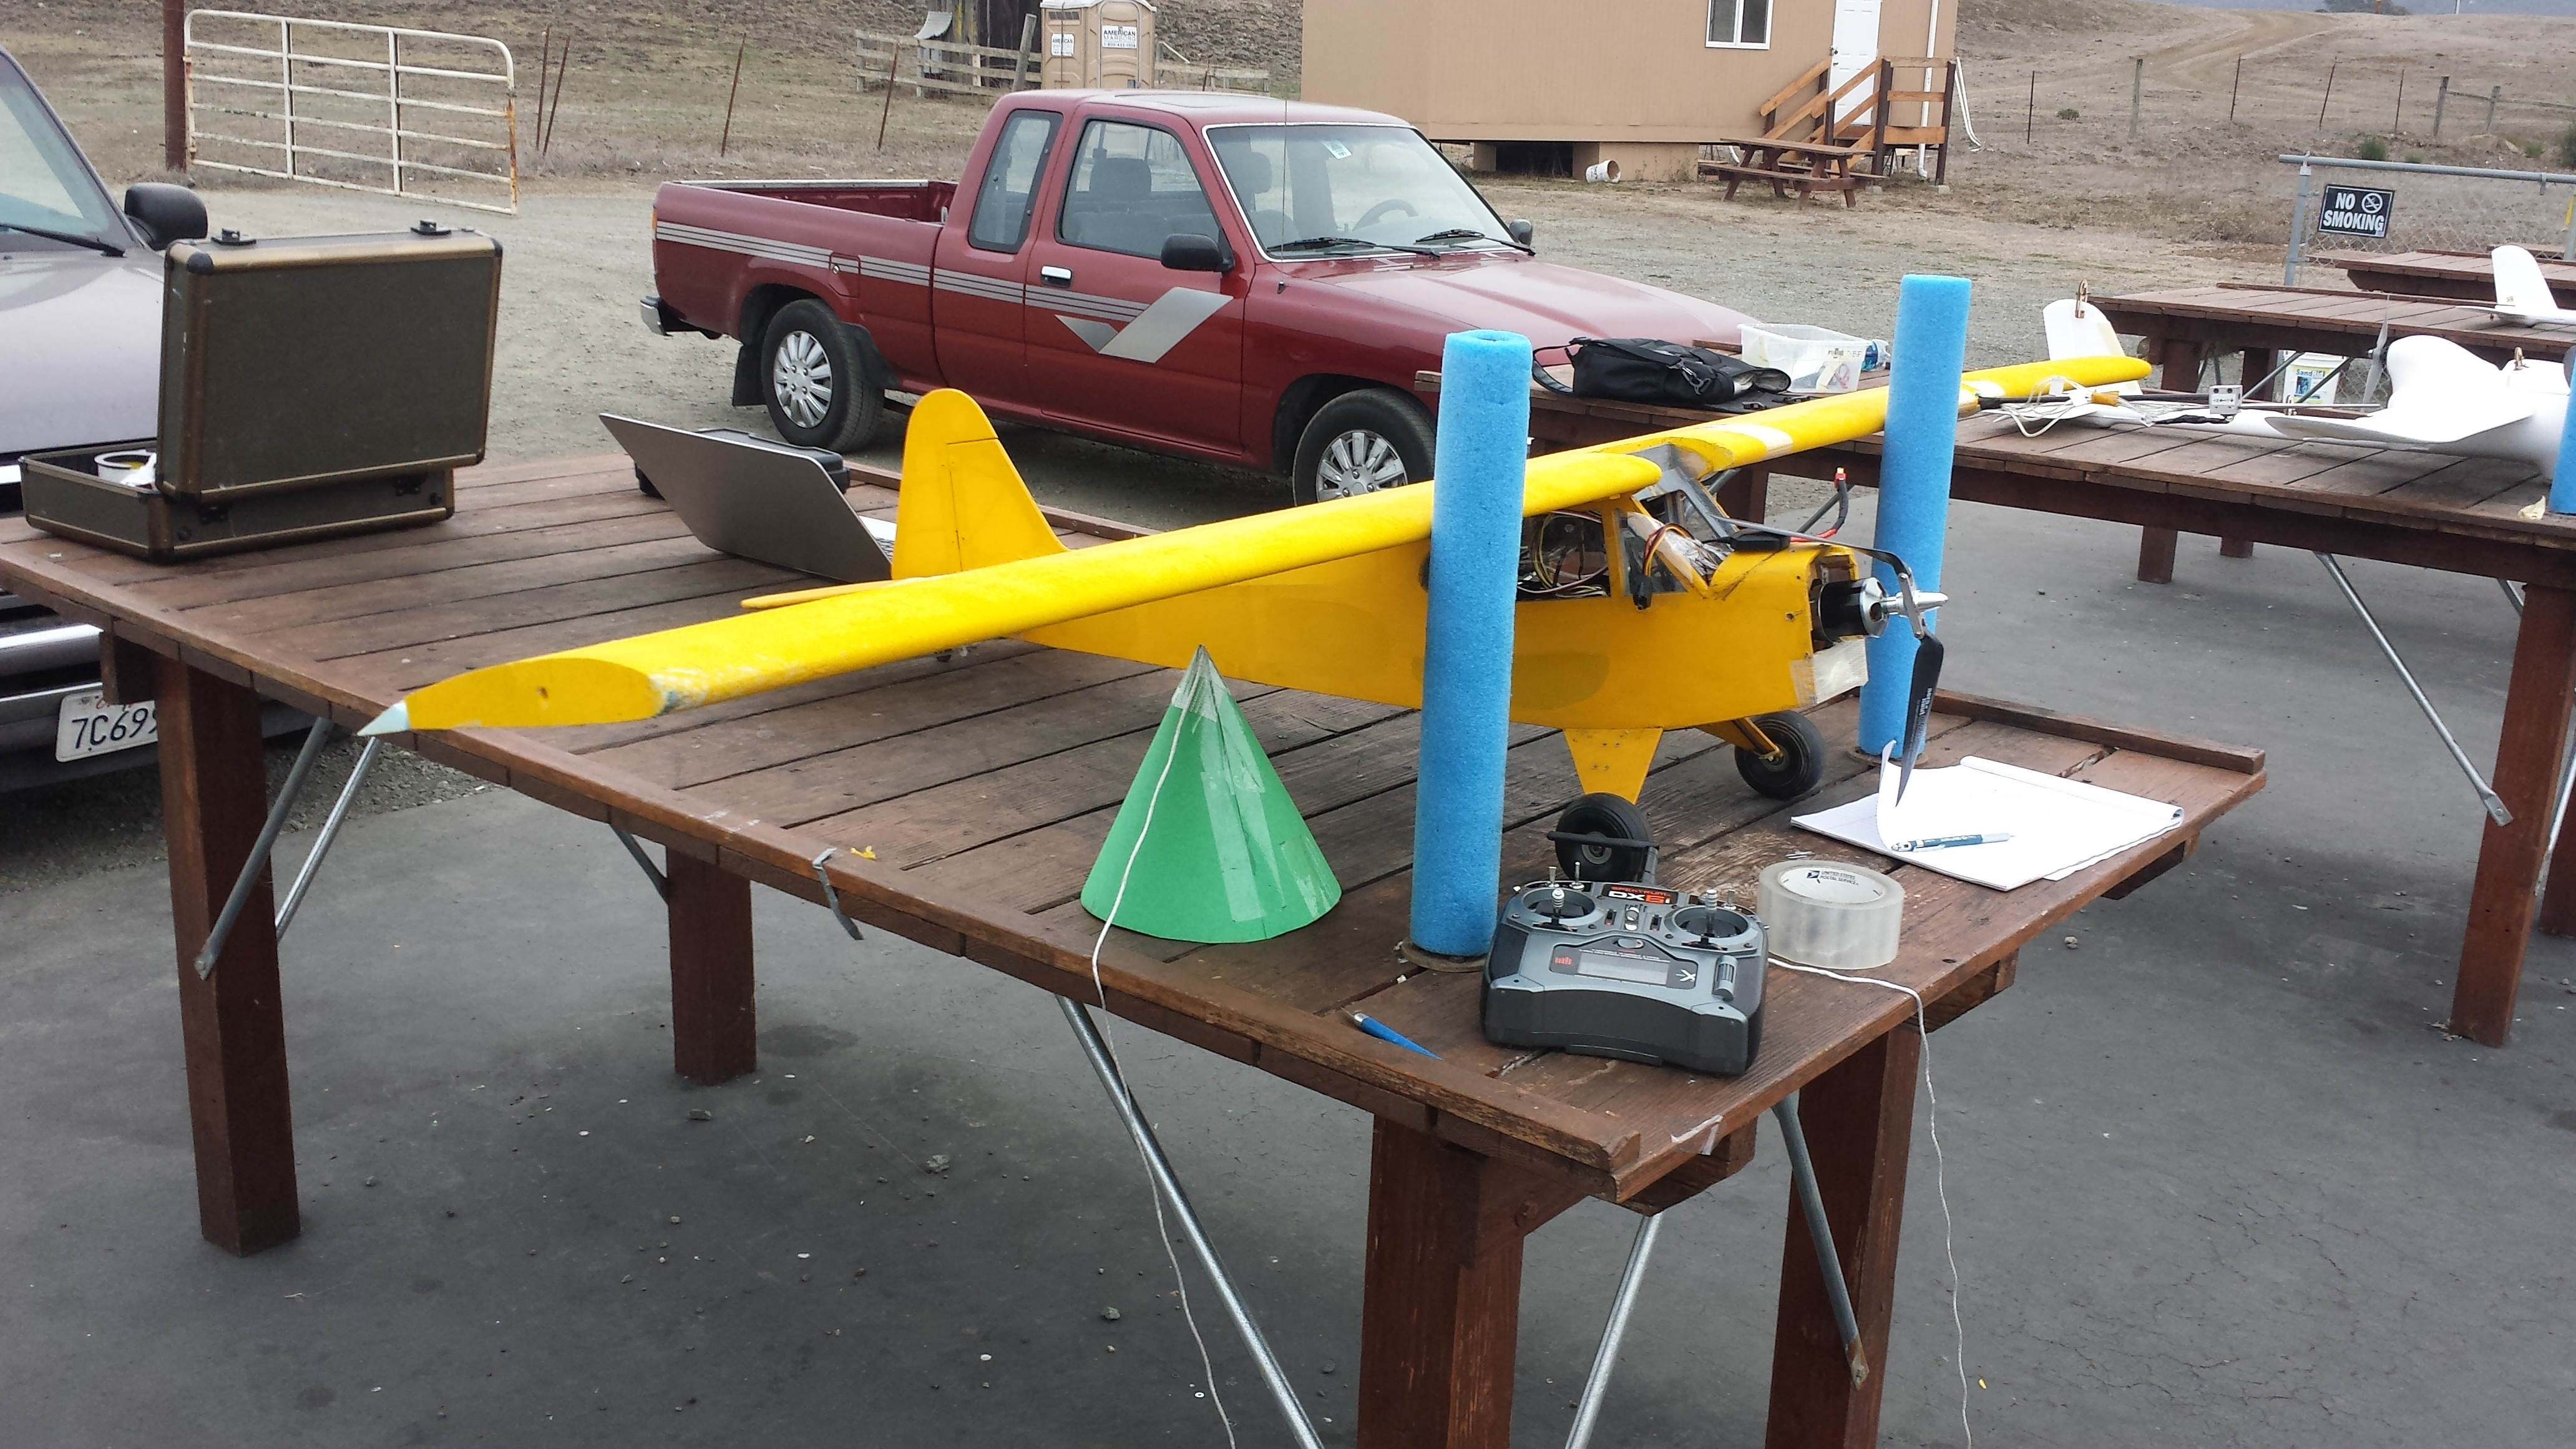
\includegraphics[width=0.9\textwidth]{figures/coneInt1.jpg}
\end{minipage}
\begin{minipage}[b]{0.45\linewidth}
  \centering
    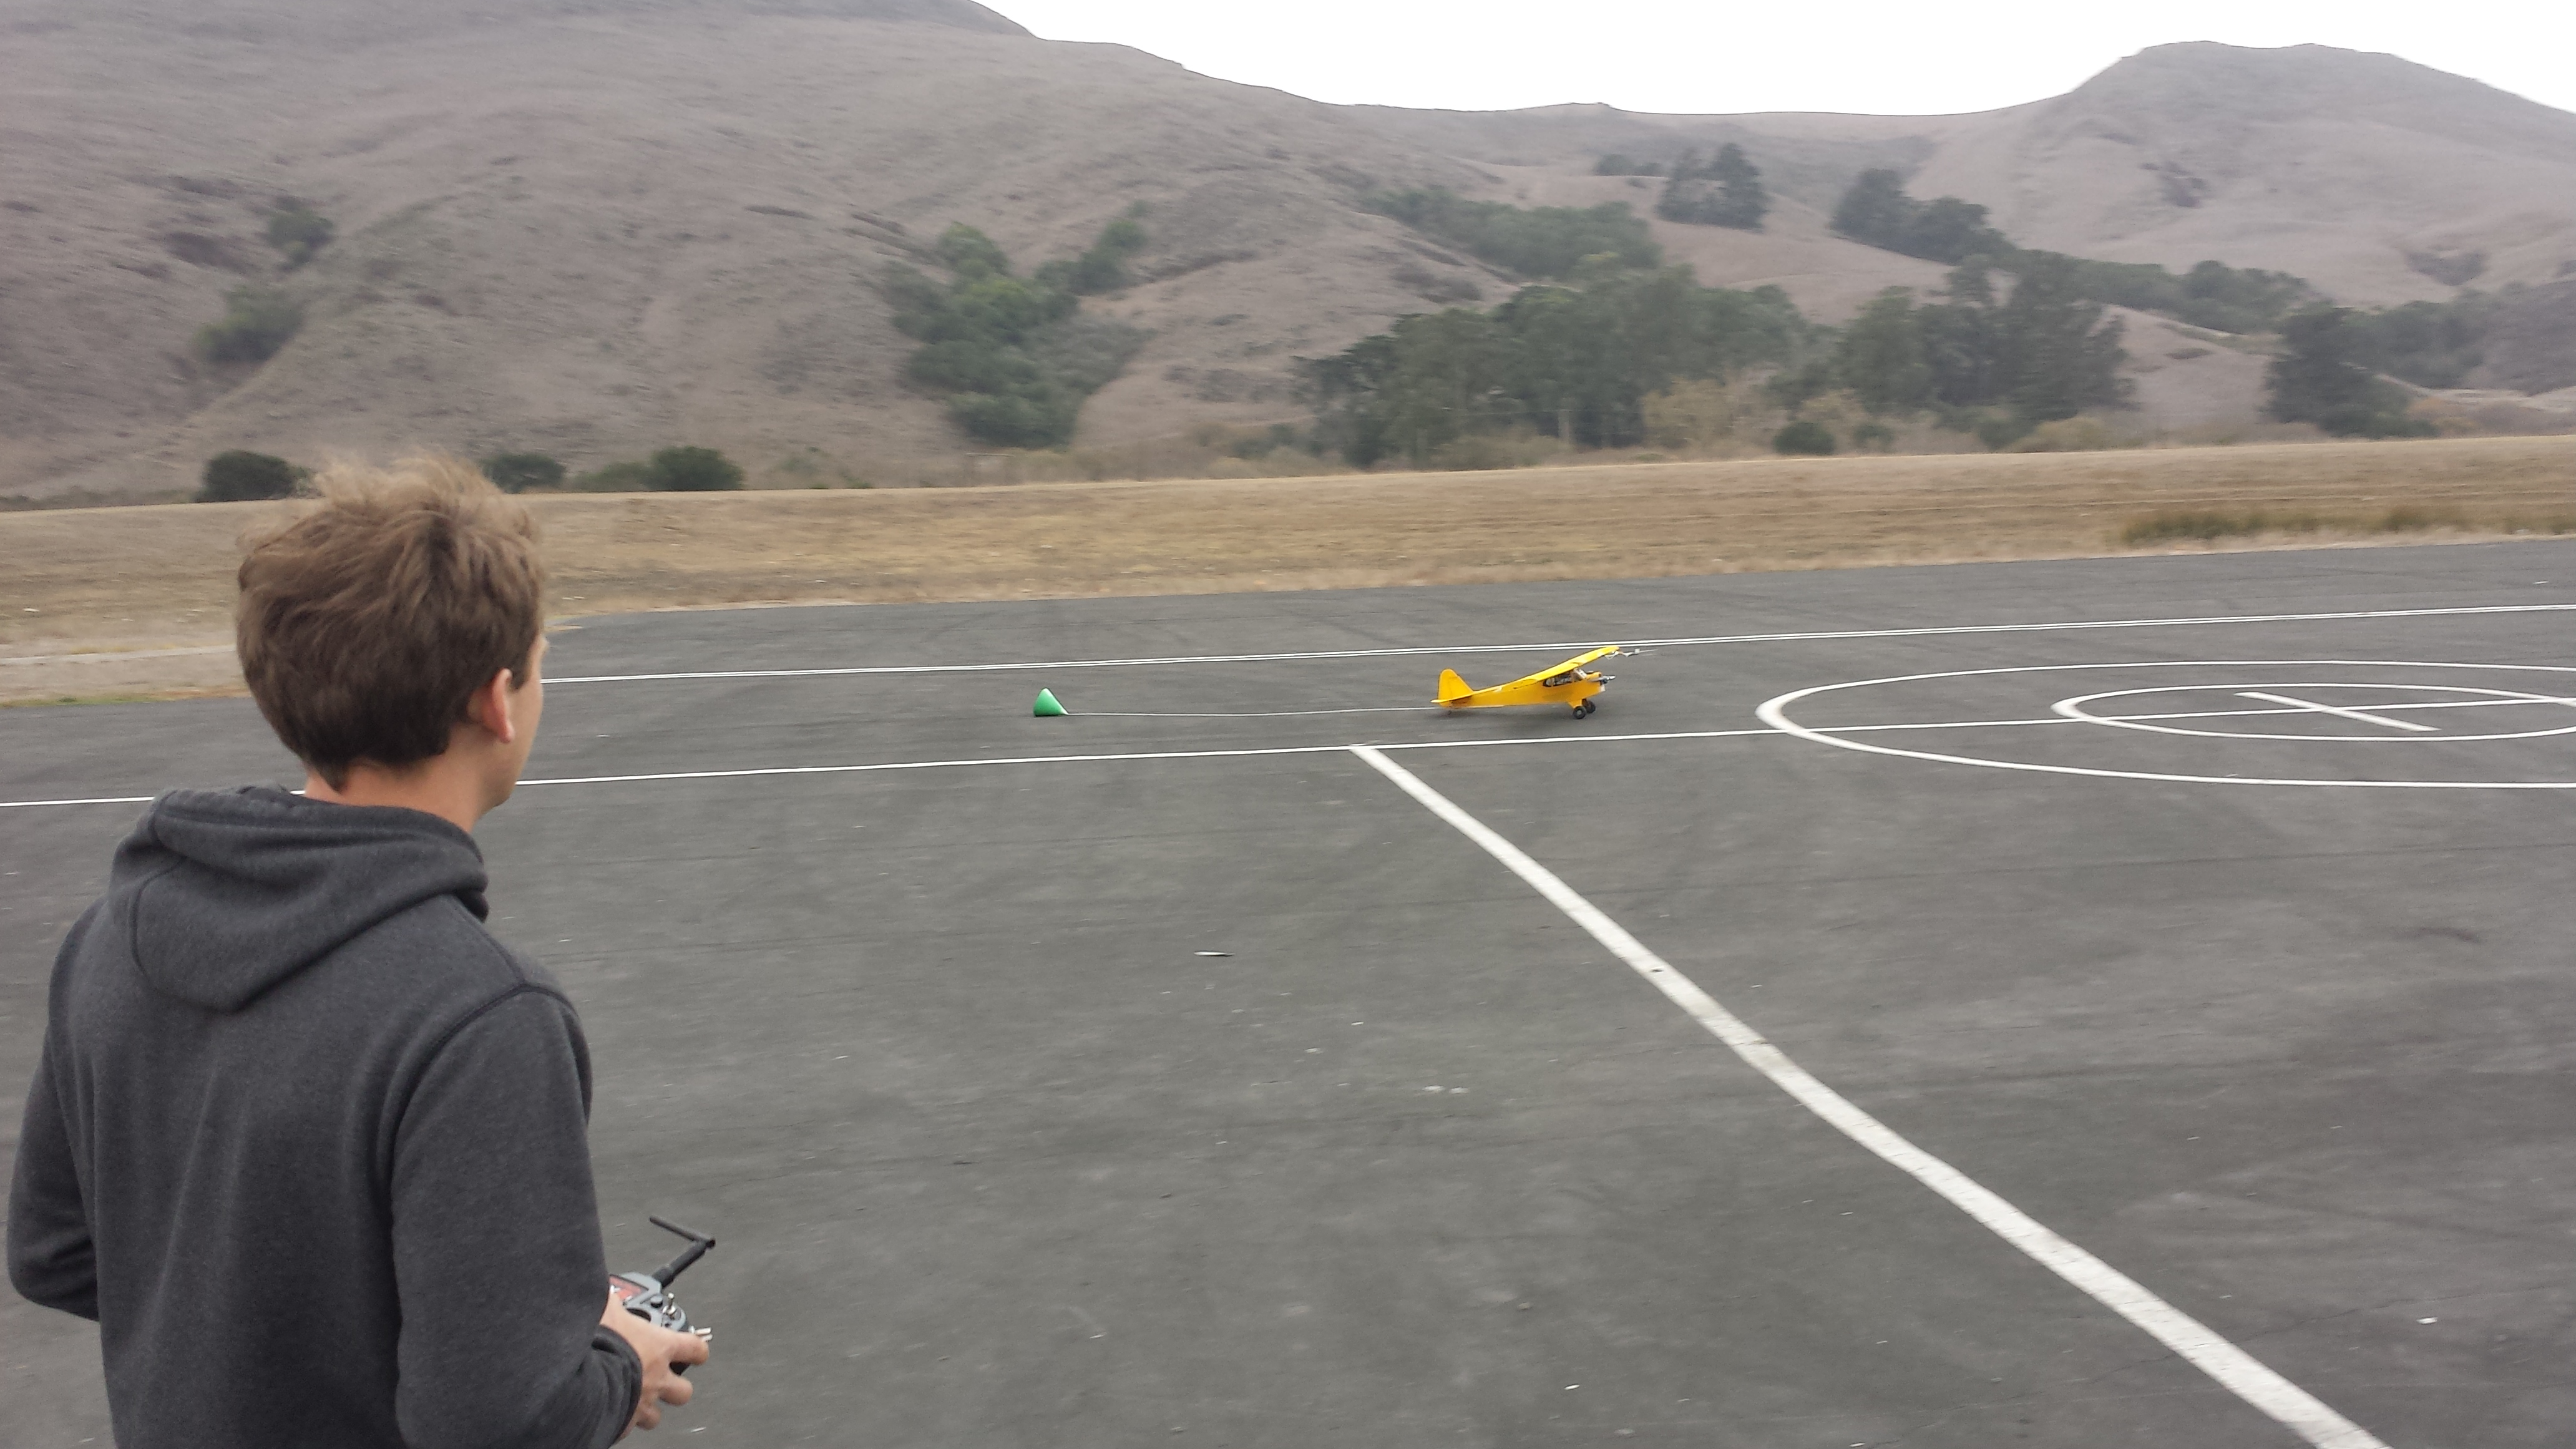
\includegraphics[width=0.9\textwidth]{figures/coneInt2.jpg}
\end{minipage}
\end{center}
\caption{Parasite Drag Cone Integration}
\label{fig:coneIntegration}
\end{figure}

The drag coefficient of a cone, as a function of its half-vertex angle, is shown in \ref{fig:coneDrag}.

\begin{figure}[H]
	\centering
	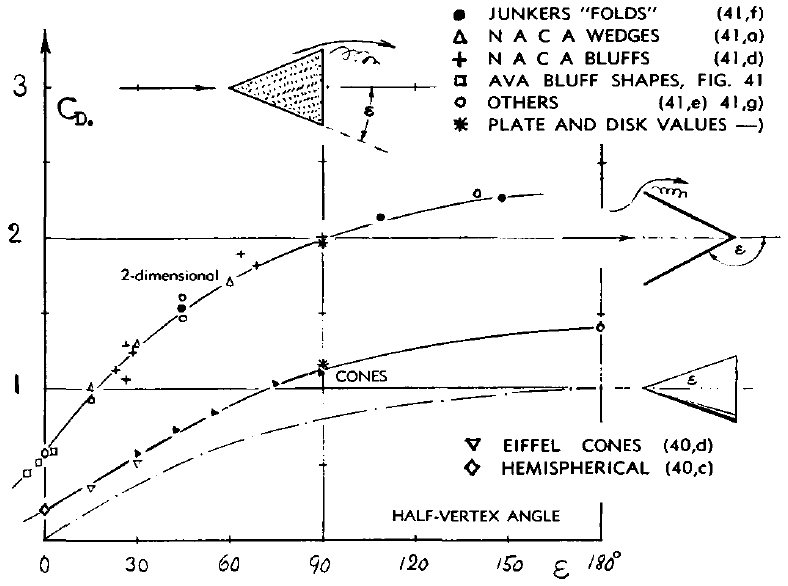
\includegraphics[width=0.7\textwidth]{figures/coneDrag.png} \caption{Cone Drag as a Function of Half Angle\cite{hoernerDrag}} \label{fig:coneDrag}
\end{figure}

	The cone was 8 inches tall and had a radius of 4.25 inches, which corresponds to a half-vertex angle of 28.0 degrees. Figure \ref{fig:coneDrag} was plot digitized, showing that a half-vertex angle of 28.0 degrees corresponded to a drag coefficient of between 0.50 and 0.56, based on the spread of the source data. For system validation, the mean of this range ($C_D = 0.53$) will be used. When scaled by the reference area, this was equal to an additional 305 counts of drag.

The system was tested three times while trailing the cone. The results are shown in Tables \ref{table:cd0RepeatDirty}-\ref{table:k2RepeatDirty}.
\newpage
\begin{table}[H]
\caption{Dirty Drag Polar Repeatability Testing : $C_{D_0}$ Regression Coefficient}
\label{table:cd0RepeatDirty}
\centering
\begin{tabular}{c c c}
\hline\hline
 Flight Number & $C_{D_0}$ Estimate & 95\% Confidence Interval \\
 \hline
4 & 0.131446 & 0.1348/0.1281 \\
5 & 0.119373 & 0.1277/0.1110 \\
6 & 0.133337 & 0.1382/0.1285 \\
\hline \hline
Combined Flights & 0.132458 & 0.1350/0.1300\\
\hline
\end{tabular}
\end{table}

\begin{table}[H]
\caption{Dirty Drag Polar Repeatability Testing : $C_1$ Regression Coefficient}
\label{table:c1RepeatDirty}
\centering
\begin{tabular}{c c c}
\hline\hline
Flight Number & $C_1$ Estimate & 95\% Confidence Interval \\
 \hline
4 & 0.004732 & 0.0087/0.0007\\
5 & 0.056782 & 0.0681/0.0454 \\
6 & 0.014184 & 0.0211/0.0072\\
\hline \hline
Combined Flights & 0.007363 & 0.0108/0.0039\\
\hline
\end{tabular}
\end{table}

\begin{table}[H]
\caption{Dirty Drag Polar Repeatability Testing : $C_2$ Regression Coefficient}
\label{table:k2RepeatDirty}
\centering
\begin{tabular}{c c c c}
\hline\hline
Flight Number & $C_2$ Estimate & 95\% Confidence Interval \\
 \hline
4 & 0.113344 & 0.1151/0.1115 \\
5 & 0.080817 & 0.0846/0.0770 \\
6 & 0.118783 & 0.1212/0.1164\\
\hline \hline
Combined Flights& 0.123563 & 0.1248/0.1223\\
\hline
\end{tabular}
\end{table}
\newpage
Figure \ref{fig:polarOverlay} shows combined drag polars for both dirty and clean configurations.
\begin{figure}[H]
  \centering
    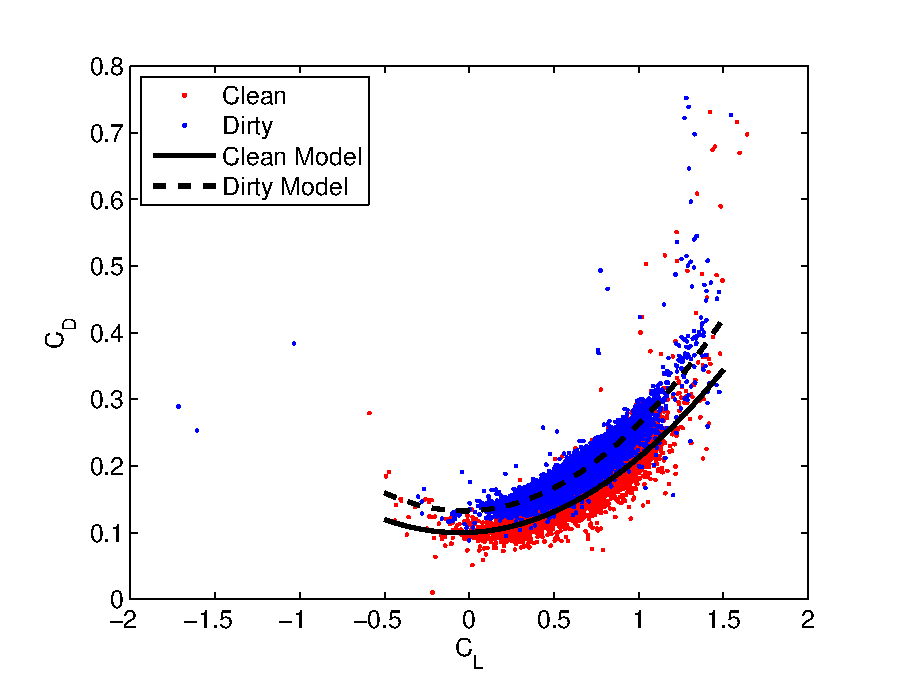
\includegraphics[width=0.7\textwidth]{figures/polarOverlay.eps}
    \caption{Clean vs. Dirty Drag Polar} \label{fig:polarOverlay}
\end{figure}

The combined regression model for the dirty configuration is shown in Equation \ref{eqn:dirtyPolar}, and the combined regression model for the clean configuration is shown in Equation \ref{eqn:cleanPolar}.

\begin{align}
C_{D_{DIRTY}} &=   0.123563 C_L^2 + 0.007363 C_L + 0.132458
\label{eqn:dirtyPolar}
\end{align}

\begin{align}
C_{D_{CLEAN}} &=   0.101002 C_L^2 + 0.011454 C_L + 0.100037
\label{eqn:cleanPolar}
\end{align}

The difference between the clean parasite drag coefficient ($C_{D_0} = 0.100037$) and the dirty parasite drag coefficient ($C_{D_0} = 0.132458$) is the contribution to the vehicle's parasite drag from the trailing cone. This amounts to $C_{D_{0,CONE}} = 0.0324$, which is 6\% higher than the value previously estimated, and well within the error of the source data.

The lift curve for both dirty and clean flight tests is shown in Figure \ref{fig:CLalphaOverlay}. The slopes are constant as is expected, since the lift curve slope is not a function of parasite drag. Note that the dirty data tends to occur at a slightly higher $C_L$ value, since the vehicle with more drag spends more time at a slower speed.
\begin{figure}[H]
  \centering
    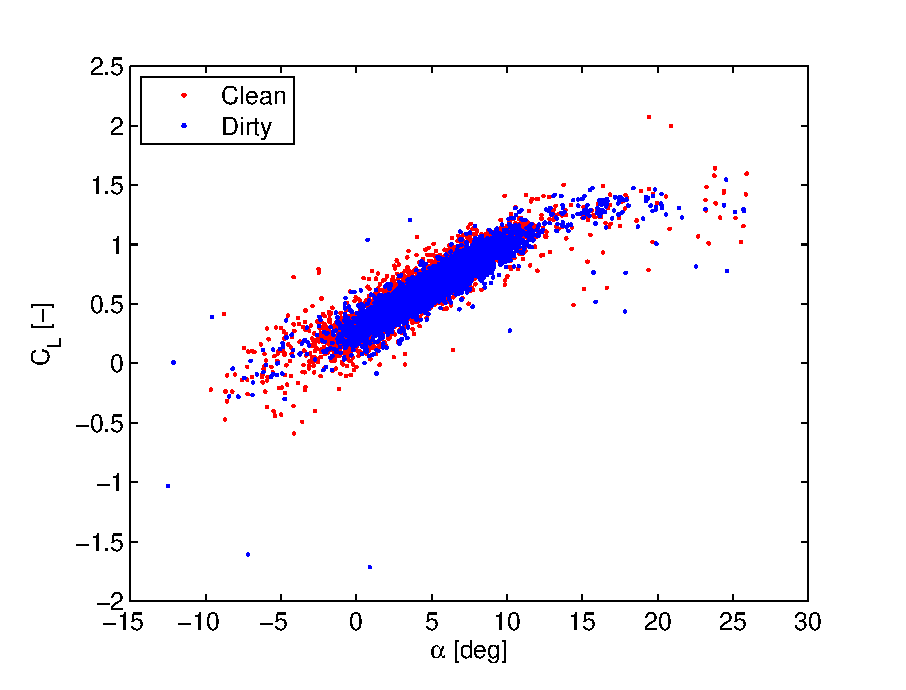
\includegraphics[width=0.7\textwidth]{figures/CLalphaOverlay.eps}
    \caption{Clean vs. Dirty Lift Curve} \label{fig:CLalphaOverlay}
\end{figure}